\chapter{低耦合、高拓展的软件综合分析系统的设计与实现}
\section{引言}
良好的软件设计应该支持软件自身更新迭代导致的各种变化\cite{Enrich2018}。随着本研究的不断深入,软件涉及的数据管理任务不断增加、需要管理维护的特征等算法不断开发、迭代、对PE进行识别判断的模型不断训练得到,这些内容都属于软件设计中
的变化。对这些内容进行有效管理需要我们设计好可以适应这些变化、具有健壮性的软件分析系统(Software comprehensive analysis system,SCAS)。同时,良好的软件设计也应该使得软件系统对类似的基于脉搏波等生理信号的各项研究有良好的兼容性与可移植性。
因此,本章着重从软件设计的角度阐述项目中涉及的具体问题及解决应对措施上的多种设计。

% 为PE分析研究而生,但不止服务于PE分析课题\cite{Enrich2018}
\section{需求分析}
一、核心分析功能

从原始生理信号中完成数据清洗、特征提取、分类模型训练和生成及最后对新数据进行有效分类是对软件分析系统最基本要求,也是软件系统应具有的核心功能。而在此功能完成的基础上,当软件系统中各个部件、模块因为种种原因
引入某种变化之后,需要根据具体情景针对该特定的变化引入代码的模式设计与重构以增加软件系统的健壮性与复用性。

二、数据源兼容

软件分析系统的使用的原始数据可能来自多种硬件采集设备自行采集或公开数据库。不同硬件设备使用的电子元器件、传感器等在性能参数上的区别可能导致PPG(在内的)数据采集质量、采样率有所差异。此外,不同的硬件厂商的导出数据存储格式也往往不尽相同。
而源自数据库的数据在字段信息上更容易出现差异。保持对不同格式数据读取的兼容性是软件分析系统需要首先解决的问题。

三、信号扩展

目前软件分析系统仅使用了1通道的光电容积脉搏波数据。但由于高性能的数据采集设备的普及,其采集得到的数据往往是多通道多参数生理信号。因此,软件分析系统需要为以后可能的多通道多生理参数的联合分析预留好设计接口,避免出现大规模的代码重构现象。

四、算法迭代与更新

在软件综合分析系统的各个环节均会使用到相应的处理算法,如数据预处理时的滤波检波算法、特征提取时的各种新型参数的计算算法以及模型训练时用到的多种机器学习模型。当需要对这些算法进行迭代更新时,特别是计算特征时又提出了新的参数,如果没有对代码进行
恰当的模式设计,很容易引发代码中大量修改与重构。

五、数据管理

从核心功能分析可以看出,本软件系统不仅需要管理原始数据,还需管理基于原始数据的参数特征。此外,由于最终生成的模型往往是基于特定数据集规模及数据集中具体参数特征,因此也需要对生成的模型进行管理。
如何对这些数据进行有效管理以及如何在不影响程序功能的情况下,增加对新数据的支持,也是软件系统需要解决的问题。此过程涉及数据的传递与保存、数据库设计及管理与预测模型的更新与管理等具体问题。

六、多场景多平台

软件分析系统需要考虑到多种潜在的应用场景,满足在实验室研究、医院监护、社区检查、居家监护多种场景下不同的使用需求。同时由于智能化设备的不断普及,软件分析系统在设计时也应该考虑到从PC端软件到移动端应用的移植与扩展的可能。

七、研究课题的扩展性

从核心功能分析可以看出,软件分析系统对PE的分析处理过程——数据清洗、特征提取、分类模型训练和生成——可以进一步抽象成一类基于人体电生理信号的分类分析过程。因此,软件分析系统在设计时应充分考虑使用将特定功能模块化,以方便对类似研究进行软件复用与扩展开发。

\section{总体方案设计}
根据上小节软件需求分析,最终实现的软件分析系统按照低耦合、高拓展的原则进行了模块化的设计:

一、客户端模块

客户端模块即数据准备模块,负责绝大部分数据处理任务,包括对数据的读取、预处理、特征计算等工作。数据处理完成后以Json的存储格式上传至服务器端,并根据上传时选择参数,由服务器训练好的数据模型返回相应的PE预测分类结果。
为方便对移动智能平台的支持,客户端模块采用静态面向对象语言Java编程完成。

二、模型训练模块

模型训练模块是软件系统的核心算法模块,需要基于提取好的数据特征完成所有模型训练、分类处理工作。由于Python在机器学习领域的广泛普及,此模块的所有编程设计与实现全部基于Python完成。训练好的分类模型也会部署至服务器端。

三、数据存储模块

数据存储模块即服务器模块,是上述两个模块的中间件,接收来自客户端的特征等数据,并将相关数据存储至数据库中,同时根据相应的特征值依据训练好的模型给出相应的预测结果。为能直接使用由模型训练模块生成的多种机器学习模型,数据存储模块采用Python为
主要编程语言,选取Django为Web框架完成服务器端相应功能的开发。

综上,软件分析系统整体设计框图如\autoref{fig:scas}所示。
\begin{figure}[htbp]
    \centering
    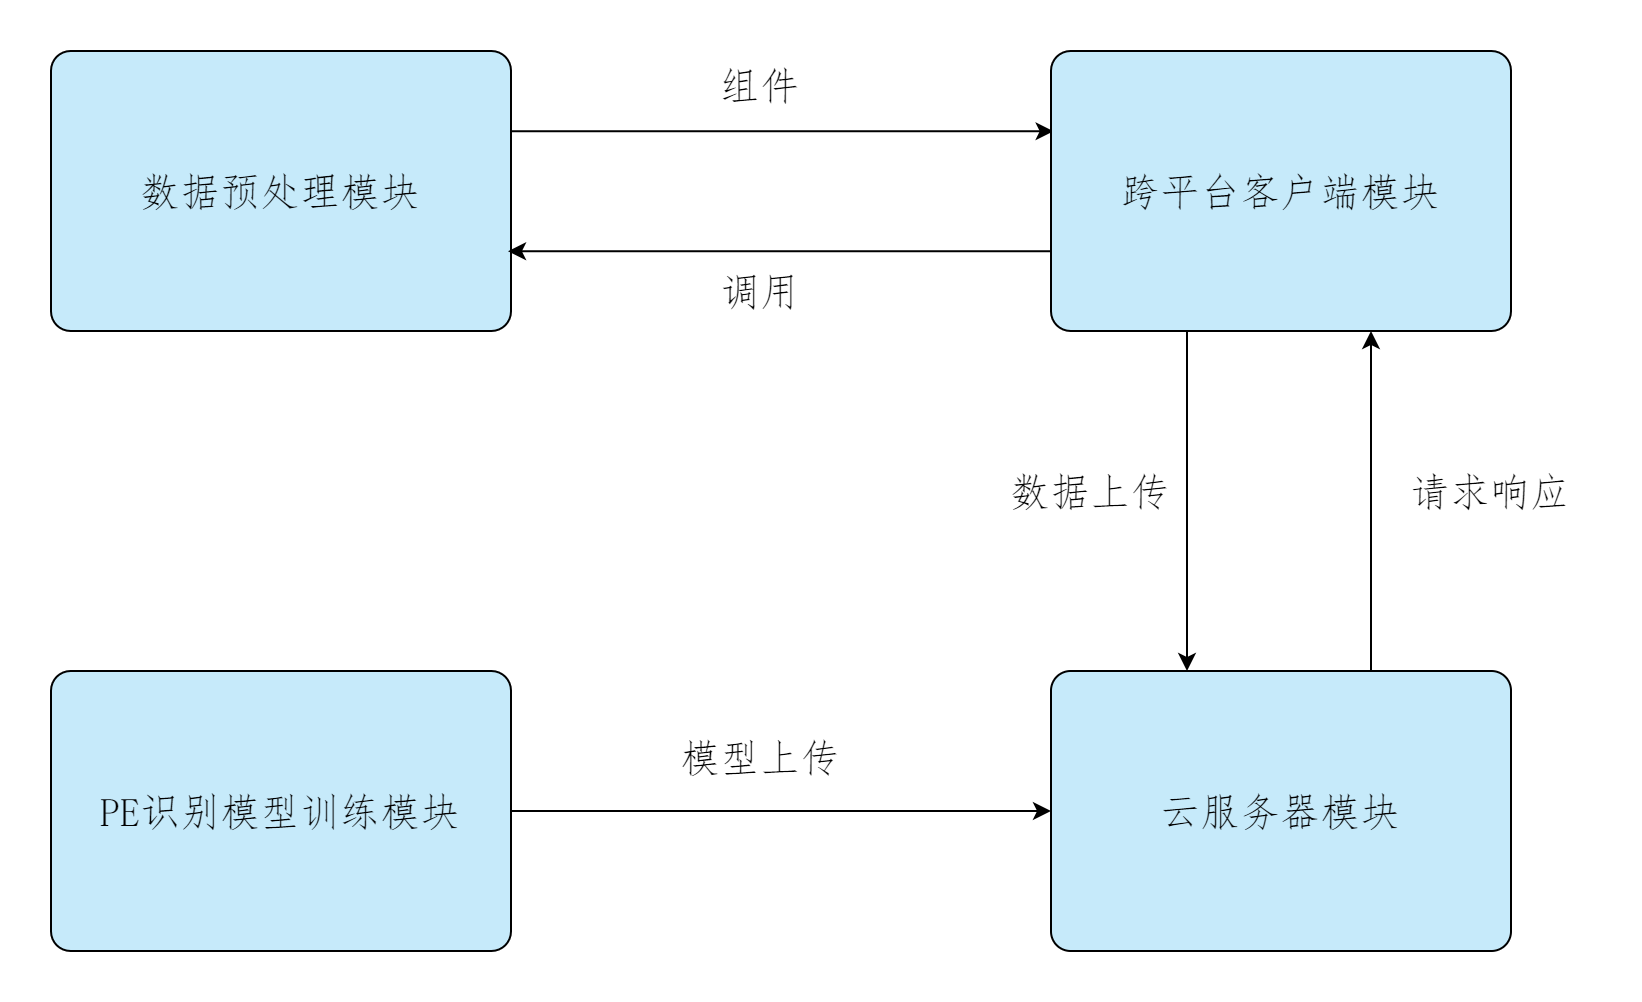
\includegraphics[width=.6\linewidth]{ch6/scas}
    \caption{\label{fig:scas}软件分析系统设计框架}
\end{figure}

\section{模块具体设计与实现}
\subsection{客户端模块}
Java是一种特殊的高级语言,兼具解释型编程语言与编译型编程语言的特性,是目前最流行的面向对象语言之一\cite{Li2015}。Java具有出色的跨操作系统平台特性,可以实现一次编译、多处使用,因此,在工业界得到了广泛应用。
此外,Java也是移动操作系统Android的主力开发语言之一\cite{android}。鉴于Java的种种优点,因此,客户端模块最终选择了Oracle开源版本的OpenJDK(16.0.2,GPLv2协议)\cite{openjdk}进行开发。在开发过程中充分利用
Java的抽象与继承特性,综合使用抽象类、接口等设计解决开发过程中出现的具体问题。

一、多种来源的数据格式的支持

本研究开展时,所有数据均来源自GE设备balabala,数据是以csv格式导出的。在研究后期,课题组也引入了迈瑞公司的 。与此同时,课题组自研多生理信号采集终端也已完成,最多可支持对127路生理信号的采集,如\autoref{fig:msd}所示。
不同厂商的硬件设备的采集得到的数据可能会有采样率、采样精度的差异,同时导出数据项也往往不尽相同。显然综合软件系统的数据读取功能需有一定的硬件适配性,
可以依据数据通讯协议、存储格式的不同灵活定制,以实现对多种硬件设备的兼容。
\begin{figure}[htbp]
    \centering
    \subfigure[连接实物图]{
    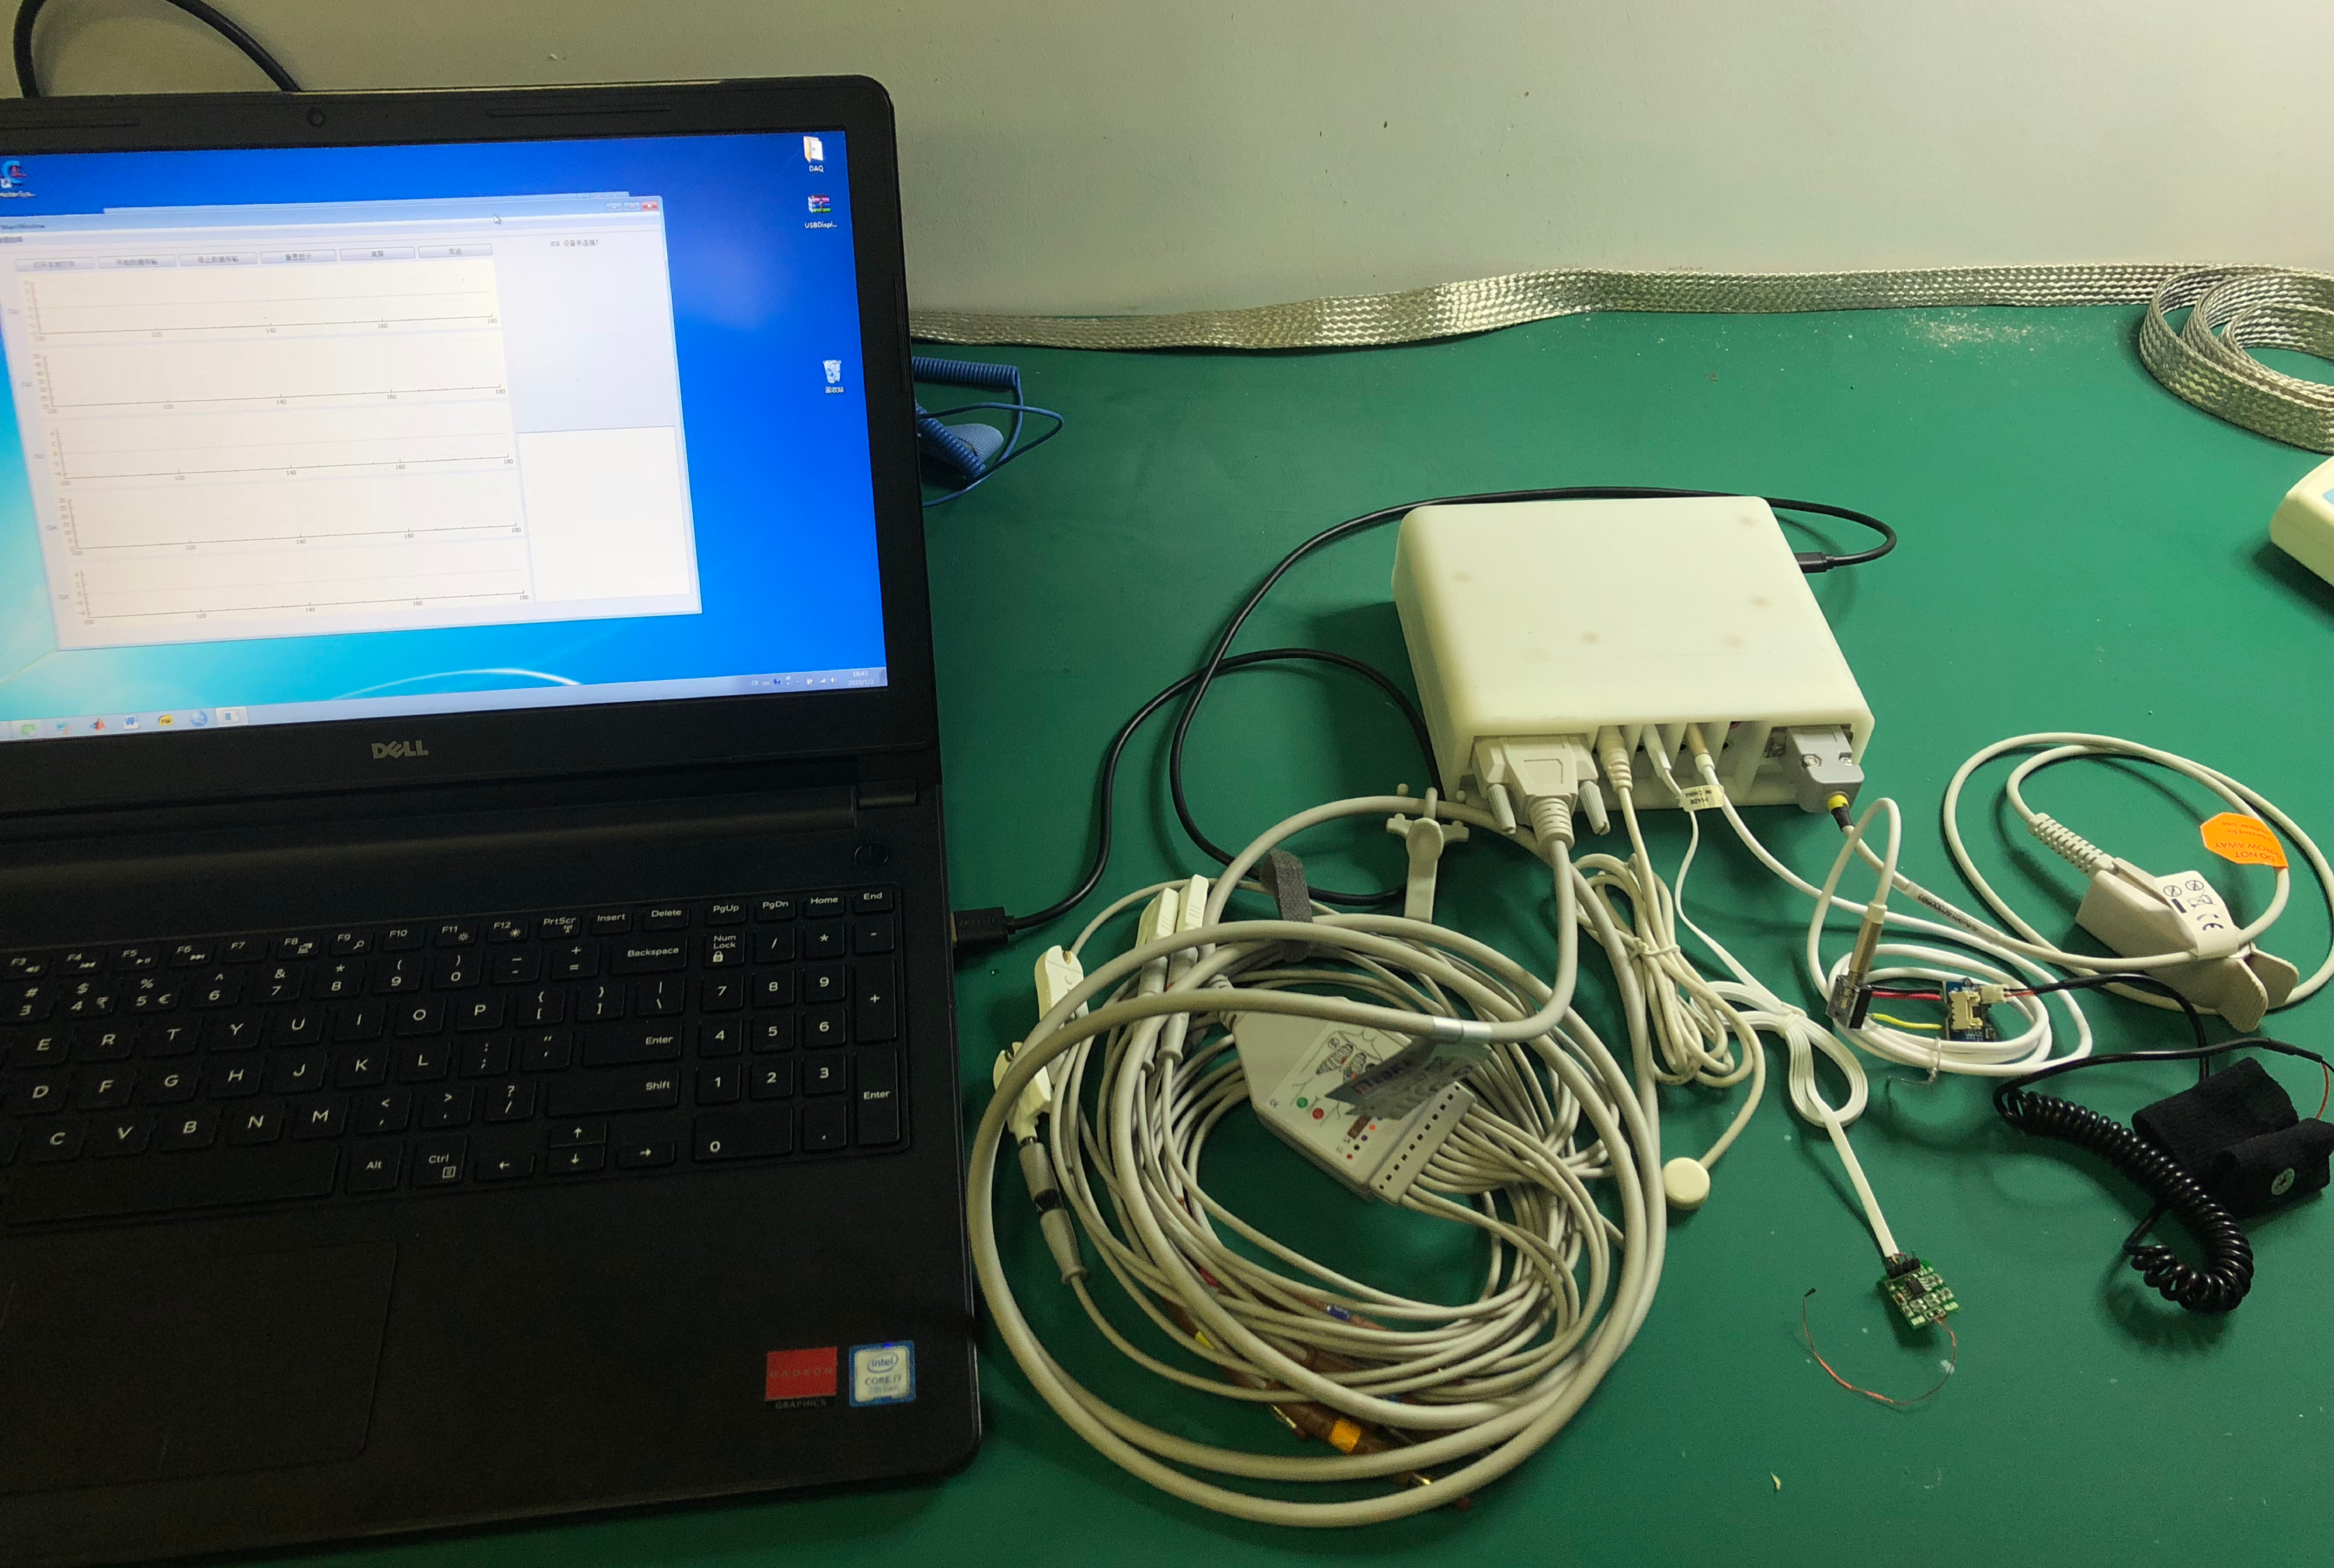
\includegraphics[width=5.5cm]{ch6/SystemCon}
    }
    \quad
    \subfigure[采集得到的信号]{
    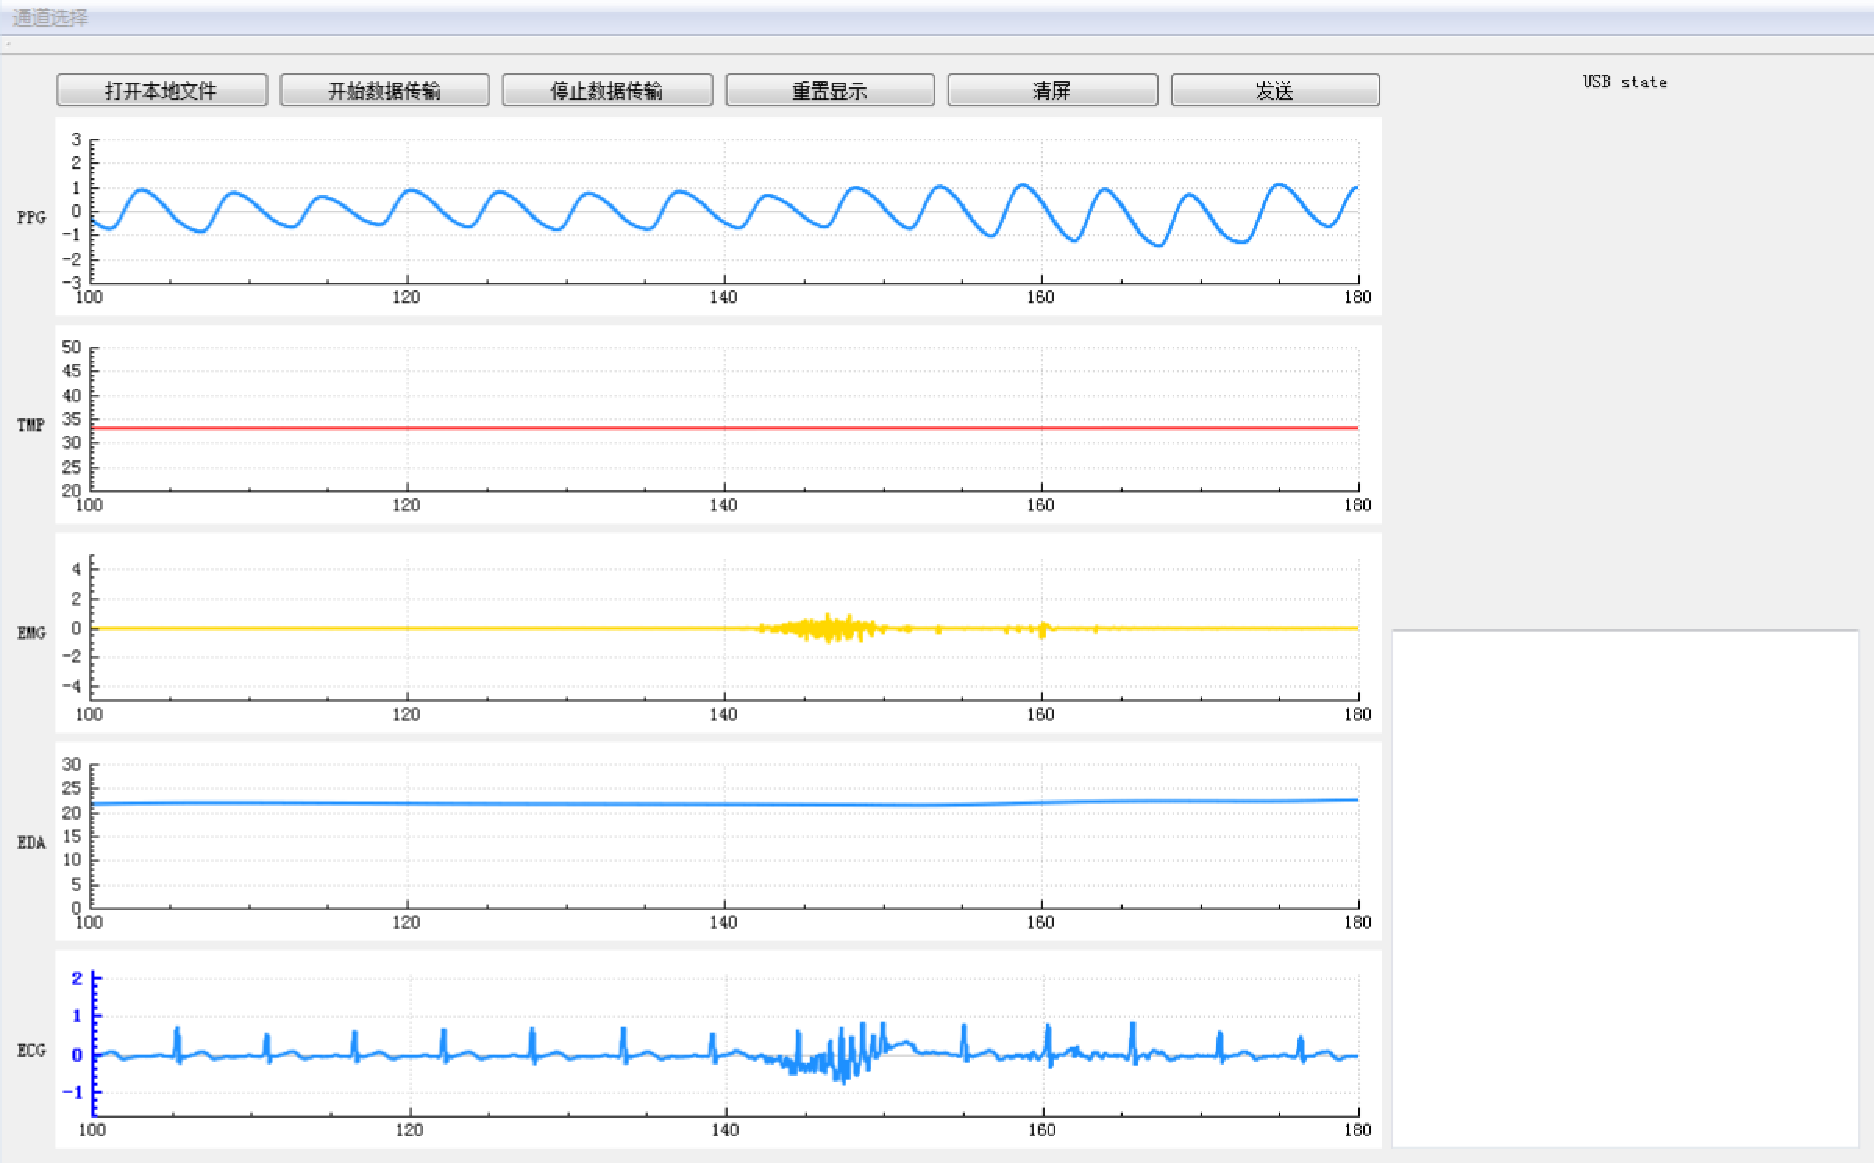
\includegraphics[width=5.5cm]{ch6/data}
    }
    \caption{\label{fig:msd}课题组自研多生理信号采集终端}
\end{figure}

为隔离由于不同硬件数据格式给数据读取模块带来的变化,在综合软件分析系统的设计中使用了规范与实现分离的机制,利用Java接口完成了所需功能。具体实现是首先将数据读取的过程定义为一抽象接口$PPGReader.class$。由于接口无法实现具体方法,因此,
当来源自某种硬件设备的数据需要进行读取时,需要一个特定的子类$SpecificReader.class$去继承该抽象接口并具体实现读取的$readFromFile.class$方法。当实现好多个与硬件绑定的子类后,需要在$TotalReader.class$类中真正读取数据时,即可按图索骥,
找到与硬件数据解析方式相对应的具体子类。这样的设计可以确保与硬件相关的特性被封装隐藏并可以随时增加新的硬件支持。这一过程中的伪代码如\autoref{lst:reader}所示。

\lstinputlisting[caption={数据读取模块的伪代码实现},label=lst:reader,style=myJava]{code/ch6/PPGReader.java}

二、预处理算法设计

数据预处理部分的软件算法工作主要由等几部分组成。由于本小节部分内容与第四章内容较为接近,预处理工作的具体实现思路可参阅前文。而数据滤波与波形检测的软件设计均采用了策略与机制分离的思想,利用工厂设计模式\cite{Enrich2018}完成。

1. 数据滤波

如前所述,在对生理信号的进行数字滤波时,一般会涉及多种类型的数字滤波器甄选。同时,每种滤波器也会有相应的可调参数。因此,性能最佳的滤波器的选择往往需要对多种滤波器调参后综合测评后才能判别,因此,软件分析系统需要能在多种滤波器之间灵活切换。

为实现上述功能,首先定义了抽象的滤波器基类$Filter.class$,在该基类中定义了滤波器的滤波、调参等基本操作的抽象方法。其次,每种特定滤波器$SpecificFilter.class$作为子类继承并实现$Filter.class$中的所有抽象方法。所有的滤波器子类并不直接实例化
,而是通过额外定义的$FilterFactory.class$这一工厂类来实现。在$FilterFactory.class$中定义好$getFilter()$方法,在该方法中选择适当的滤波器种类,将其实例化后,根据实际需求调整好滤波器性能参数并返回该实例。另一方面,当主程序中需要使用
滤波器对原始信号进行处理时,仅需调用$FilterFactory.class$的$getFilter()$方法即可。任何对滤波器种类及相关参数的设置与修改对主程序而言均是不可见的,从而很好的隔离了滤波器设置对主程序代码的影响,降低了软件系统的耦合性。
这一过程中的伪代码如\autoref{lst:filter}所示。
\lstinputlisting[caption={滤波器设置的伪代码实现},label=lst:filter,style=myJava]{code/ch6/PPGReader.java}

2. 波形检测

脉搏波波形检测是本研究的基础,波形检测算法的准确性将直接影响后续分析工作。此前的研究人员已经提出过多种脉搏波波形检测方式\cite{Wang2012},本文则在前人基础上进一步优化了波形检测的流程,将之前的一次性检测改成了检测-复核-决策(Detect-Check-Keep)
的反馈式检波流程,进一步提高了脉搏波波形检测准确性,该过程中的流程图如\autoref{fig:check}所示。
\begin{figure}[htbp]
    \centering
    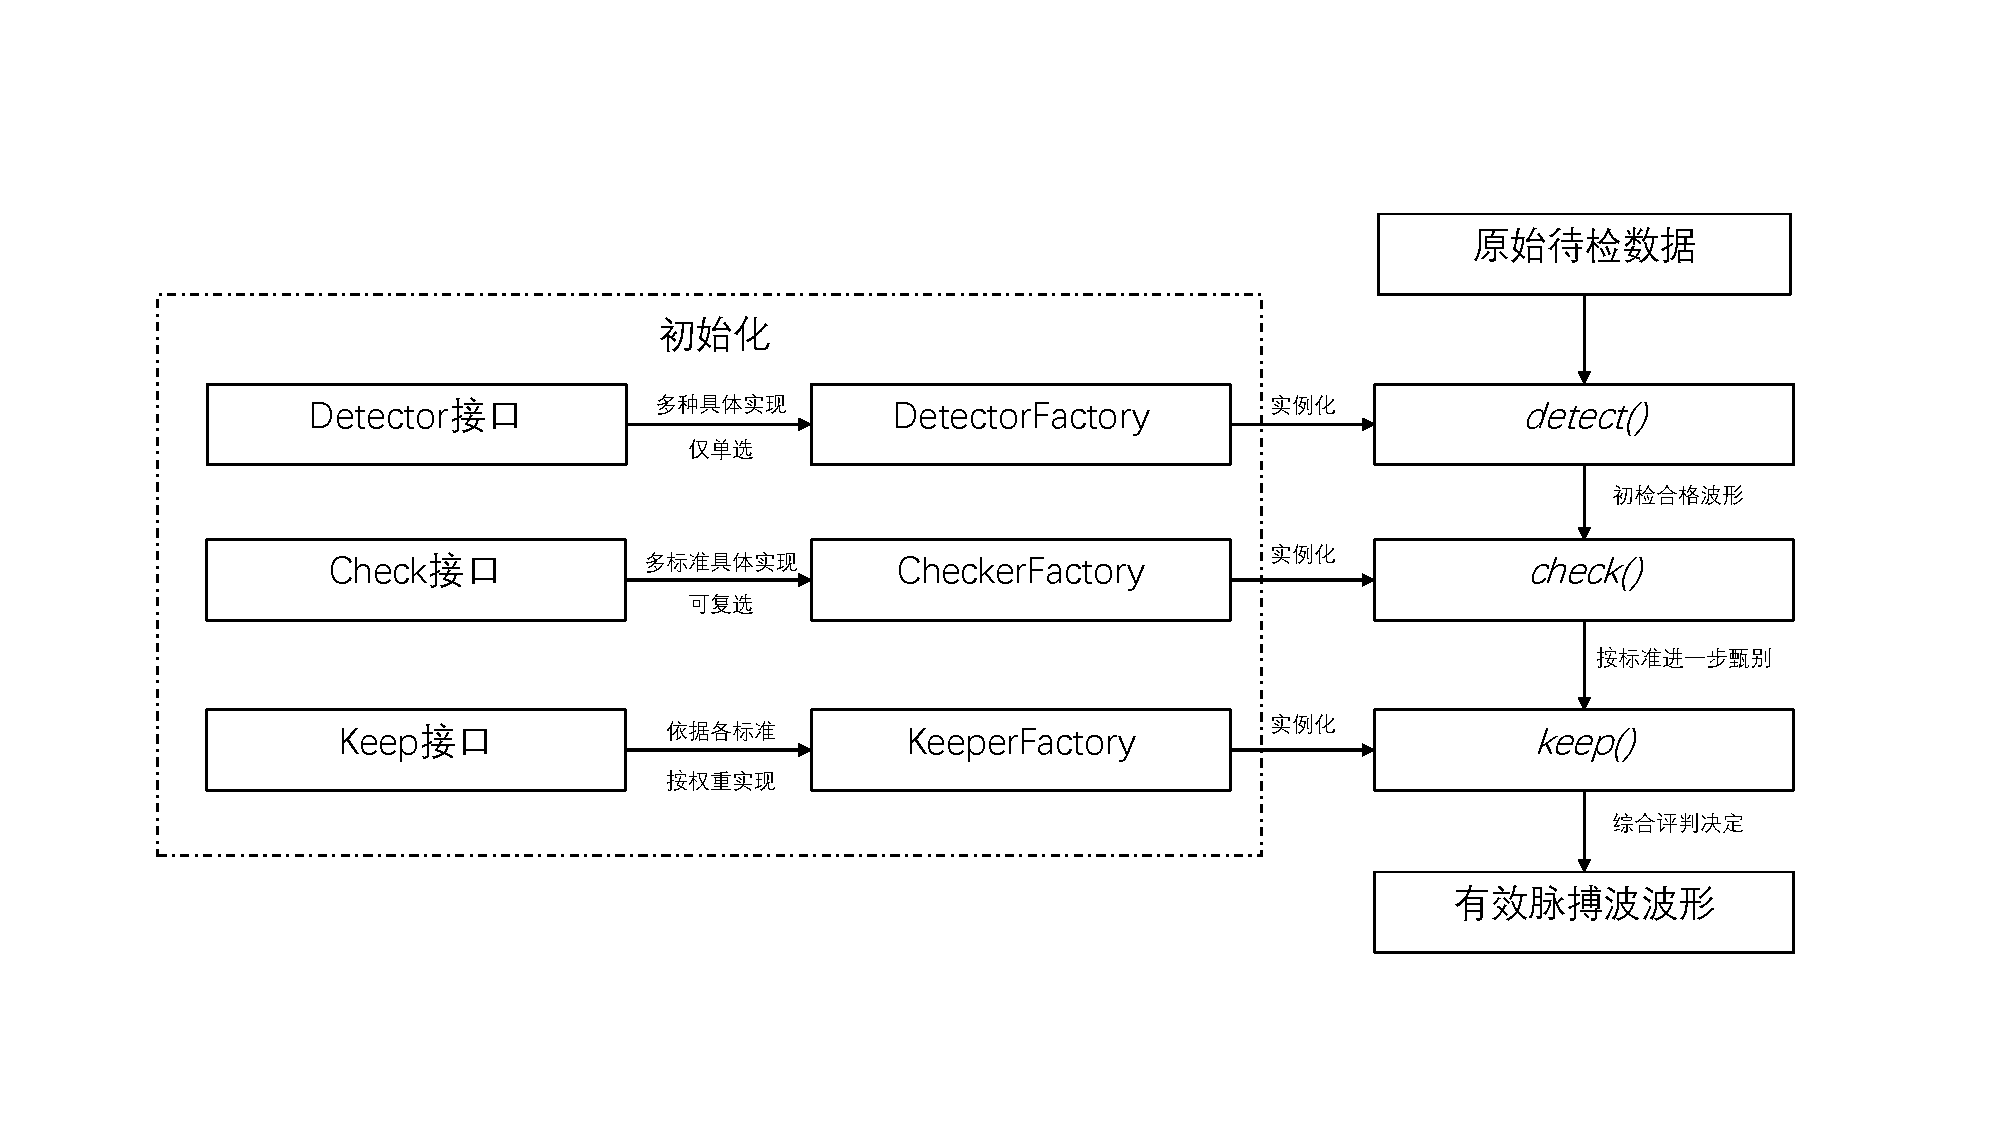
\includegraphics[width=1.1\linewidth]{ch6/check}
    \caption{\label{fig:check}改进后的检波流程图}
\end{figure}

其中,$detect()$方法负责按照一定的基础规则初步筛选出所有可能脉搏波波形位置。$check()$方法则遵循一定的标准,对初筛的结果进一步复核,筛选出某些不符合标准的疑似误检的波形。其中,本研究中自行定义了一些复核标准,
包括如两个波形的间期需在合理时间内、同一人的脉搏波波形在短时间内波形应较为接近、单个脉搏波波形的能量不应与所有波形的平均能量有较大的出入等。随后$keep()$方法则负责对$check()$的结果进行综合评判,可按照投票决策或比重决策等方式来决定最终判断疑似误检波形的
去留。最后,在初筛的波形中剔除误检的波形则可得到最终的检测结果。

与上小节中的数字滤波的工厂模式设计类似,Detector、Checker及Keeper分别是检波算法、复核算法及决策算法的基类,分别定义了各算法的基本行为,但不负责实现具体功能。具体的实现算法需要重新定义子类继承相应的基类,
并实现其中的相应的$detect()$、$check()$及$keep()$方法。此时,再分别定义各算法的工厂类,将各算法实例化过程进行封装。其中,需要注意的是,$DetectorFactory.class$与$KeeperFactory.class$返回的实例都仅含有一个对象,而$CheckerFactory.class$
可以返回包含多个实例的集合,即同时返回多个复核标准同时对初筛结果进行检测。

上述设计可以有效提高脉搏波波形检测的准确性,并且可以按需求灵活定制筛选标准、调整检波精度。与此同时,根据实际需要和检波效果等因素,检测算法的Detector、Checker及Keeper等部分均可自行改动、调整、优化,且不影响主程序中的代码执行,从而实现了
检波算法的各环节的高内聚性及算法与系统整体之间的低耦合性。

三、信号特征算法设计

基于脉搏波的波形检测算法无疑是客户端软件的核心功能之一,且是客户端软件中改动变化最频繁、最容易因代码的更迭而发生增删修改的部分。降低特征算法的更迭对客户端软件的整体影响,是对特征算法整体设计的基本要求。本研究中,对特征算法
的整体设计如\autoref{fig:features}所示。
\begin{figure}[htbp]
    \centering
    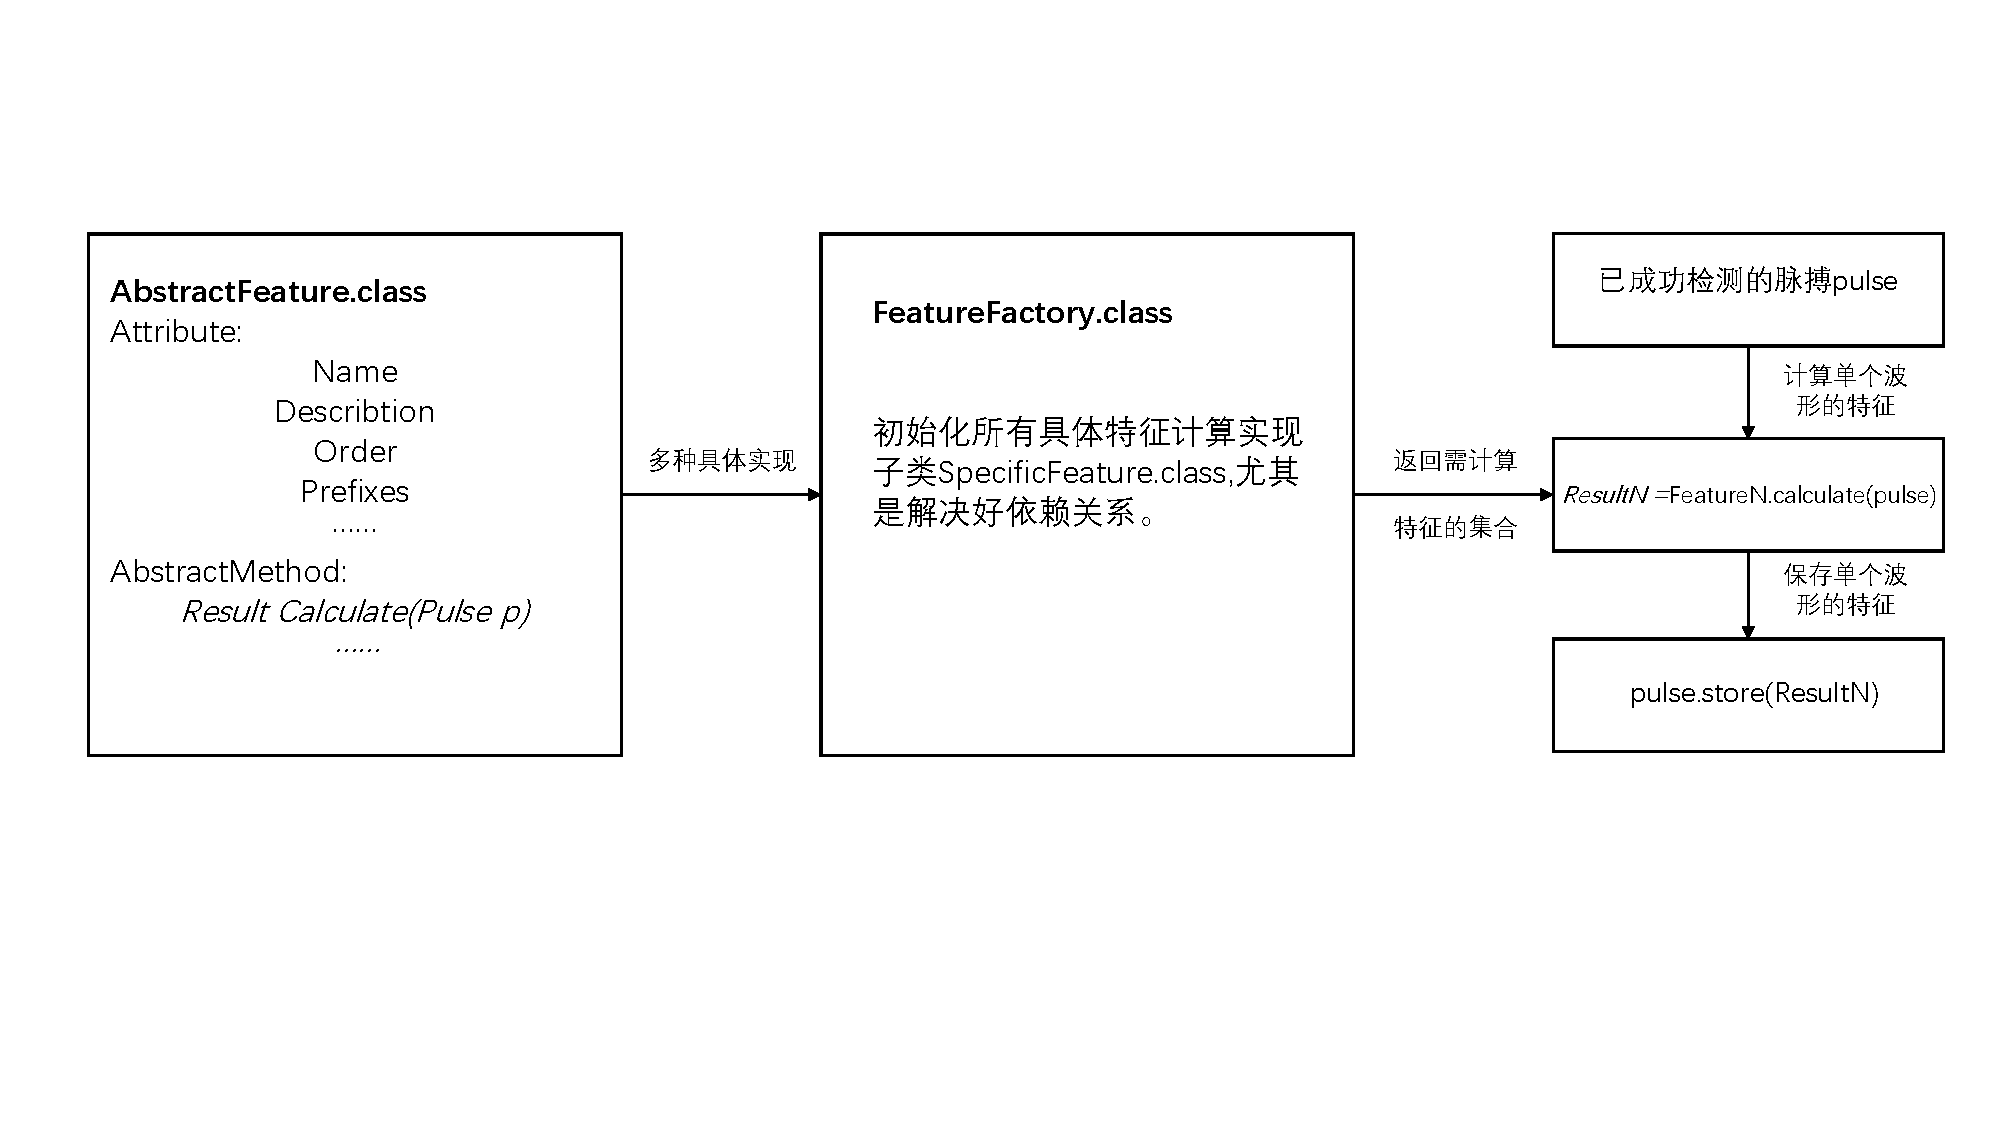
\includegraphics[width=1\linewidth]{ch6/feature}
    \caption{\label{fig:features}特征计算的算法流程图}
\end{figure}

与前小节的设计类似,$AbstractFeature.class$是个抽象父类,规定了所有特征应有的一般属性,包括特征名及其缩写$Name$,特征所代表的含义$Describition$等描述信息。而在$AbstractFeature.class$的子类$SpesificFeatureX.class$中才根据具体设计思想等完成对
该特征的计算过程$calculate()$。值得注意的是,在\autoref{fig:features}中,$AbstractFeature.class$额外定了两个属性$Order$与$Prefixes$。
这是因为某些特定的特征在计算时,可能需要一定的先导条件,即需要预先计算好一定的先导特征。因此,每个特征在初始化时,按照先导条件从无到有、从少到多、从简单到复杂的原则,给每个具体实现子类$SpesificFeatureX.class$设置好其计算顺序
$Order$及保存着其先导特征$Order$的$Prefixes$,最后按照所有子类$SpesificFeatureX.class$的$Order$遍历,即可保证所有特征均按指定顺序全部计算完毕。

而上述先导设置过程,可以在$SpesificFeatureX.class$定义时设定,但为了保持更多的调整灵活性。最终在实现软件系统时额外定义了$FeatureFactory.class$,用以集中完成并封装所有需进行计算的特征子类的初始化工作。而在主程序中调用$FeatureFactory.class$
的$GetAllFeatures()$方法时,其返回值将是包含所有特征子类的列表,并特征子类的$Order$值决定了该子类在返回列表里的排列顺序,即真正的执行顺序。若软件系统需要增加某一新型特征算法,只需设计新的$SpesificFeature.class$,实现其具体的计算过程,
随后在$FeatureFactory.class$设置好对应$Order$与所需的$Prefixes$等在内的初始化工作,即可完成对待检特征集的拓展。

此外\autoref{fig:features}也给出了特定脉搏波波形所有特征的具体计算流程。首先,客户端需完成数据预处理工作,获取所有待计算的脉搏波完整波形。其次,通过实例化$FeatureFactory.class$并调用$GetAllFeatures()$方法以获取所有待计算的特征集合。
随后,针对特征集合里面的每个$SpesificFeatureX.class$特征,分别调用其$calculate()$方法完成计算。此时特定波形的具体特征值仍然保持在$SpesificFeatureX.class$中,故最后,需要将结果保持至该波形对应的具体$Pulse.class$实例中,
即执行最后的$pulseX.Store(feature)$操作。另外,不难发现,$FeatureFactory.class$的实例化过程会随着待检波形的更迭而不断进行,最终会导致Java虚拟机重复创建、同时消耗系统内存资源。为减少该冗余操作,
最后客户端使用了设计模式中的Singlon单例模式\cite{Li2015}对$FeatureFactory.class$
进行了再次设计,即只可以创建一个$FeatureFactory.class$的实例,此后所有调用$FeatureFactory.class$的创建方法只会返回第一次调用时创建的实例。

四、多种数据类型的支持

尽管现阶段针对PE的研究主要基于脉搏波这一生理信号,但并不排除更多人体生理信号会增加进信号分析的可能。而上述过程中,涉及的脉搏波原始数据读取、预处理及信号特征设计与计算等过程也可以作为生理信号的一般处理过程。
鉴于此,客户端软件进一步设计了$AbstractBMESignal.class$这一抽象类来表征一般生理信号,数据读取、预处理及信号特征计算过程均设计成抽象方法,$Pulse.class$是继承该抽象类的复杂处理脉搏波信号的子类。若有其他生理信号的分析需求,可以视情况
拓展实现心电$ECG.class$、脑电$EEG.class$等,这一过程如所示。

五、数据导出

当客户端完成对生理信号的分析后,如何将分析处理结果进行保存是客户端软件最后需要解决的问题。导出的数据是以检测的PPG波形为基础,包含该波形所有形态特征。而在本研究中,多种新设计的特征参数往往是以向量的形式出现,因此最后导出的结果将会大量出现波形——
特征——向量(pulse-feature-vector)这种二级树状结构。此外信号特征算法出现引入了新的信号特征、对已有特征值数值的保存形式进行更改等更迭将会直接引起数据存储格式的变化。而常见的基于列表式的cvs、txt等对这种树状数据格式的支持较差,
需要借助新的数据储存格式来实现。

扩展标记语言(Extensible Markup Language,XML) \cite{xml,Li2016}与JavaScript对象标记法(JavaScript Object Notation,JSON)\cite{json,Crockford2006}是两种服务器端流行的数据交换格式。两者均可按照实际需求灵活定制存储规则,对较为复杂的数据结构
支持性好、拓展性强。但由于XML是基于标签描述数据的,在描述数组类型数据时,引入了大量冗余信息。而JSON则对数组类数据有着更好的支持,有着更快的读写速度与更高的存储效率\cite{Nurseitov2009}。因此,软件分析系统最终使用JSON作为数据交换格式,
而在具体实现时使用了中国阿里巴巴公司的开源JSON解析库fastjson\cite{fastjson}进行编码。最后的导出数据如\autoref{lst:json}所示,除基本数据特征外,与数据相关的文件信息及孕妇人口统计学信息也被保存至JSON文件。
\lstinputlisting[caption={导出数据示意},label=lst:json,style=myJava]{code/ch6/out.json}
% \begin{figure}[htbp]
%     \centering
%     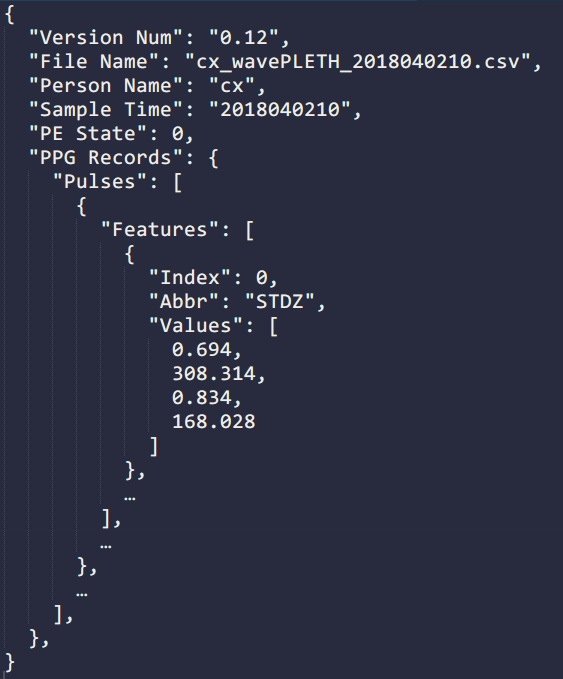
\includegraphics[width=.6\linewidth]{ch6/json}
%     \caption{\label{fig:json}导出数据示意}
% \end{figure}

六、多平台支持

综合考虑软件实际的使用场合与应用前景,本研究最终选择了对Windows PC平台及Andoird移动平台进行了适配开发。由于Java的天然的跨平台特性,前文提及的多项软件设计在实现后可直接在PC端与移动端顺利运行。另一方面,Android系统独立于Java社区,主要由美国Google公司
负责维护及更新,因此经常会出现某些Java组件在PC端与Android端的生命周期不一致的现象,并直接导致部分PC端可用的Java组件在新版本的Android系统下不被支持。因此,软件系统的特定功能需要针对具体操作系统平台选取恰当的组件完成功能开发。图\autoref{tab:platform}
展示了PC端与Android移动端相同软件功能在具体实现组件上的差异。由于此过程中较少涉及算法模式的设计,故正文对具体开发实现过程不再赘述。
\begin{table}[htbp]
    \centering
    \fontsize{10}{6}
    \caption{\label{tab:platform}Windows与Andoird平台下部分软件功能使用的开发组件对比}
    \begin{tabularx}{\linewidth}{X<{\centering}X<{\centering}X<{\centering}}
        \toprule \textbf{功能特征}&\textbf{Windows}&\textbf{Android}\\
        \midrule 
        数据上传&HttpClient\cite{HttpClient}&Retrofit\cite{Retrofit}\\
        数据图表显示&JFreeChart\cite{JFreeChart}&MPAndroidChart\cite{MPAndroidChart}\\
        \bottomrule
    \end{tabularx}
\end{table}

七、UI界面

1. PC界面

\autoref{fig:pc_ui}展示了软件分析系统在PC上运行效果。可通过文件菜单选择对原始数据的打开及经分析后特征数据的导出。编辑菜单可以完成数据的预处理、分析等功能。帮助菜单则给出软件开发单位、软件版本号等信息。软件
的主界面展示了打开数据文件的波形图,可以通过鼠标完成拖动、缩放等功能。对波形的波峰波谷等特征点的分析也在图中有所标示。右键菜单同时还提供了修改绘图颜色字体属性,支持选中当前波形直接复制至文件及连接打印机打印等功能。
\begin{figure}[htbp]
    \centering
    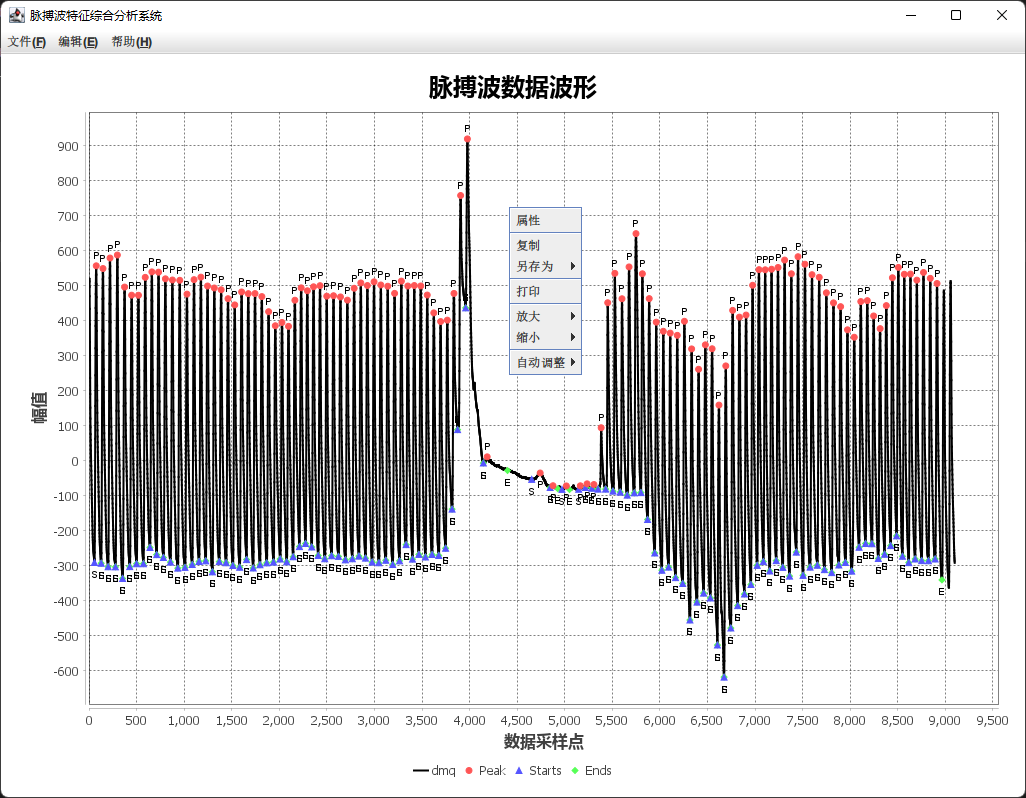
\includegraphics[width=.8\linewidth]{ch6/pc_ui}
    \caption{\label{fig:pc_ui}PC软件运行界面}
\end{figure}

2. Android界面

\autoref{fig:aui}展示了软件分析系统在Android上运行效果。
\begin{figure}[htbp]
    \centering
    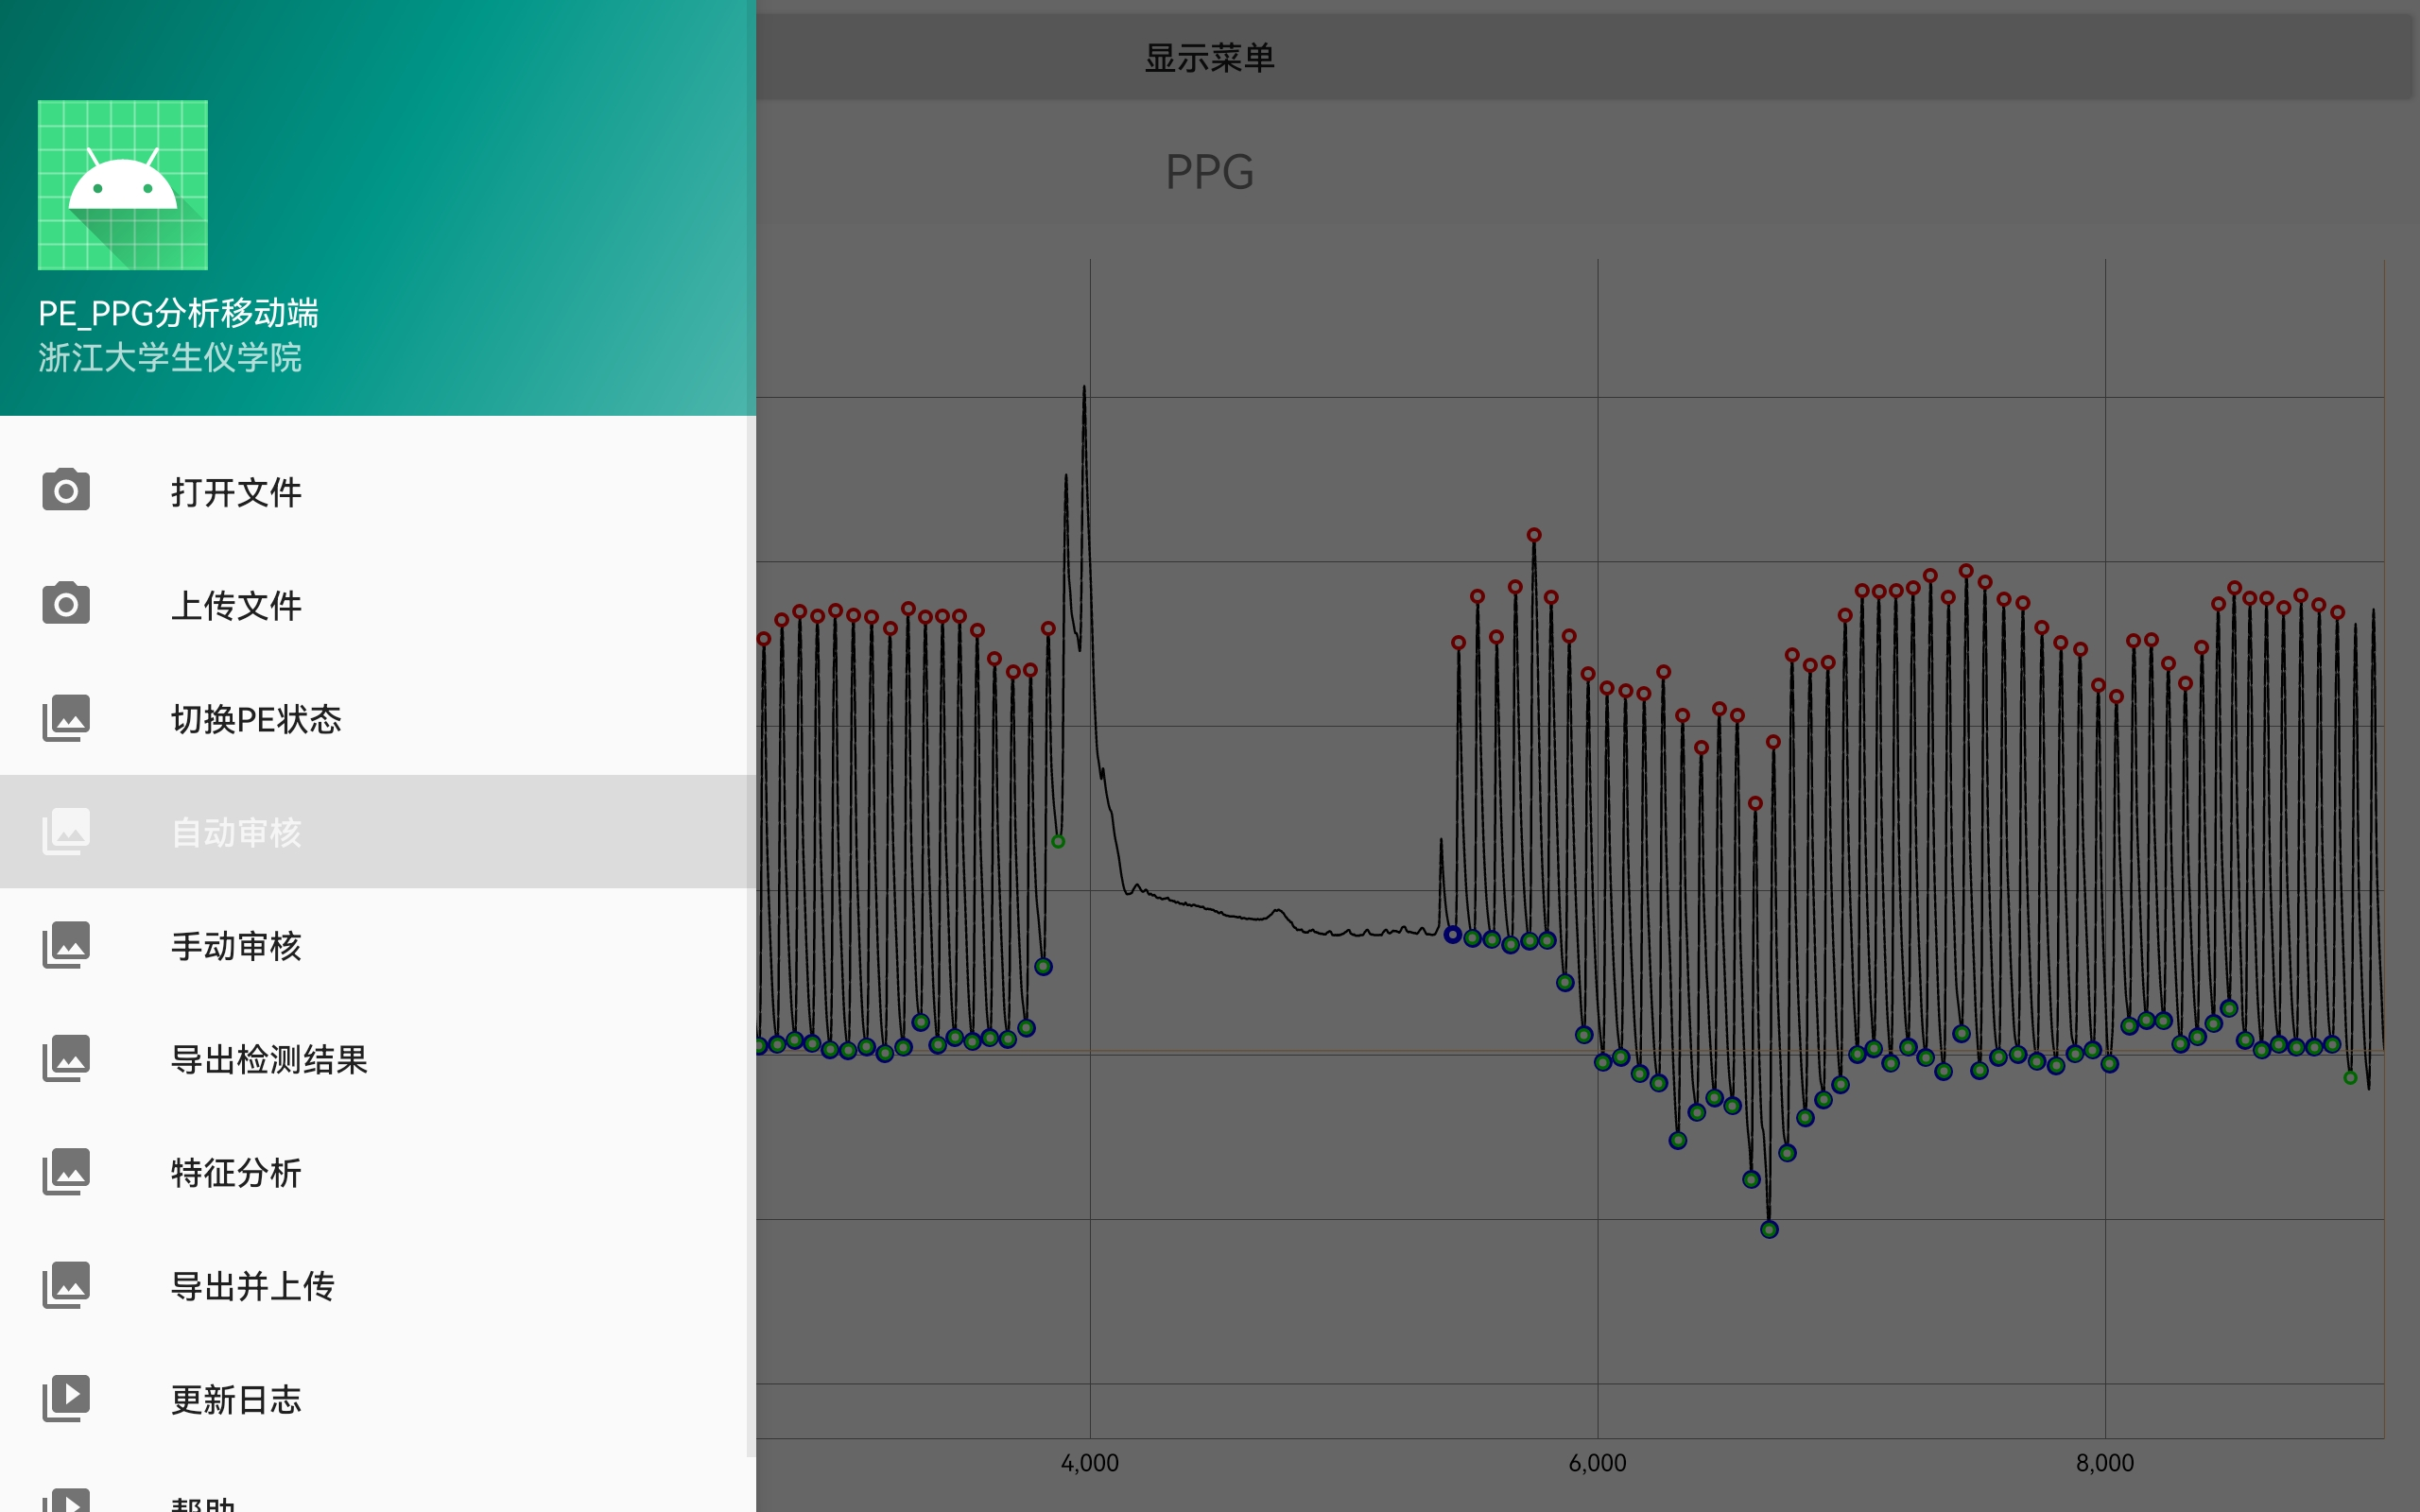
\includegraphics[width=.8\linewidth]{ch6/android_ui}
    \caption{\label{fig:aui}Android软件运行界面}
\end{figure}

\subsection{服务器模块}

一、数据库设计

二、模型存储设计

三、模型调用设计

\subsection{模型训练模块}
一、数据获取

二、模型训练

\section{系统验证与测试}
界面
输入输出
\section{小结}